%!TEX root = ../main.tex

This chapter describes the setup of the case study.
The \cref{fig:casestudy-workflow} depicts the overall workflow of this thesis.
In the following sections each step is elucidated.
Strong emphasis is laid on numbers and decisions.

\begin{figure}[ht]
  \centering
  \smartdiagramset{back arrow disabled=true,
    text width=.6\textwidth,
    uniform color list=black!40 for 5 items}
  \smartdiagram[flow diagram:vertical]{
    {Determine companies, keywords and stock symbols to analyze},
    {Gather data},
    {Normalization of tweets},
    {Determine sentiment of tweets},
    {Comparing sentiment time series with share prices}
  }

  \caption{Workflow of this thesis}
  \label{fig:casestudy-workflow}
\end{figure}

\section{Determine companies, keywords and stock symbols to analyze}
\label{s:casestudy-companieskeywords}

First, a list of automotive companies is needed.
These companies must be traded on a stock exchange to perform the comparison with tweet sentiments.
As a single company may own several car brands a list of all brands has been set up.
The result of the analysis is depicted in \cref{tab:casestudy-brands}.
Both brands which aren't customer facing passenger car brands and brands which do not longer exist have been omitted.
Furthermore, the brands have been grouped by their owning company.

  \begin{longtable}[c]{!l ^l}
    \hline
    \rowstyle{\bfseries}
    Car brand & Owning Company  \\ \hline
  \endfirsthead
  %
  \multicolumn{2}{c}%
  {{\bfseries Table \thetable\ continued from previous page}} \\
   &  \\
  \endhead
  %
  BMW  & BMW \cite[p.30]{BMWGroup2017} \\
  Mini  & BMW  \cite[p.30]{BMWGroup2017} \\
  Rolls-Royce   & BMW \cite[p.30]{BMWGroup2017} \\
  Mercedes-AMG & Daimler \cite[p.90]{DaimlerAG2018} \\
  Mercedes-Benz  & Daimler \cite[p.90]{DaimlerAG2018} \\
  Mercedes-Maybach & Daimler \cite[p.90]{DaimlerAG2018} \\
  Smart  & Daimler \cite[p.90]{DaimlerAG2018} \\
  Alfa Romeo & Fiat Chrysler Automobiles \cite[p.32]{FiatChryslerAutomobiles2018a} \\
  Chrysler & Fiat Chrysler Automobiles \cite[p.32]{FiatChryslerAutomobiles2018a} \\
  Dodge & Fiat Chrysler Automobiles \cite[p.32]{FiatChryslerAutomobiles2018a} \\
  Fiat & Fiat Chrysler Automobiles \cite[p.32]{FiatChryslerAutomobiles2018a} \\
  Fiat Professional & Fiat Chrysler Automobiles \cite[p.32]{FiatChryslerAutomobiles2018a} \\
  Jeep & Fiat Chrysler Automobiles \cite[p.32]{FiatChryslerAutomobiles2018a} \\
  Lancia & Fiat Chrysler Automobiles \cite[p.32]{FiatChryslerAutomobiles2018a} \\
  RAM & Fiat Chrysler Automobiles \cite[p.32]{FiatChryslerAutomobiles2018a} \\
  Ford & Ford Motor Company \cite[p.18]{FordMotorCompany2018} \\
  Lincoln  & Ford Motor Company \cite[p.18]{FordMotorCompany2018} \\
  Baojun & General Motors Company \cite[p.1]{GeneralMotorsCompany2018} \\
  Buick & General Motors Company \cite[p.1]{GeneralMotorsCompany2018} \\
  Cadillac & General Motors Company \cite[p.1]{GeneralMotorsCompany2018} \\
  Chevrolet & General Motors Company \cite[p.1]{GeneralMotorsCompany2018} \\
  GMC & General Motors Company \cite[p.1]{GeneralMotorsCompany2018} \\
  Holden & General Motors Company \cite[p.1]{GeneralMotorsCompany2018} \\
  Jiefang & General Motors Company \cite[p.1]{GeneralMotorsCompany2018} \\
  Wuling & General Motors Company \cite[p.1]{GeneralMotorsCompany2018} \\
  Honda & Honda \cite[p.3]{HondaMotorCo.2017} \\
  Hyundai & Hyundai Motor Company \cite[p.127]{HyundaiMotorCompany2016} \\
  KIA & Hyundai Motor Company \cite[p.127]{HyundaiMotorCompany2016} \\
  Datsun & Nissan Motor Corporation \cite[p.5]{NissanMotorCorporation2017} \\
  Infinity & Nissan Motor Corporation \cite[p.5]{NissanMotorCorporation2017} \\
  Nissan & Nissan Motor Corporation \cite[p.5]{NissanMotorCorporation2017} \\
  Citroën & Groupe PSA \cite[p.3]{GroupePSA2018} \\
  Opel & Groupe PSA \cite[p.3]{GroupePSA2018} \\
  Peugeot& Groupe PSA \cite[p.3]{GroupePSA2018} \\
  Vauxhall & Groupe PSA \cite[p.3]{GroupePSA2018} \\
  Alpine & Groupe Renault \cite[p.11]{GroupeRenault2018} \\
  Dacia & Groupe Renault \cite[p.11]{GroupeRenault2018} \\
  Lada & Groupe Renault \cite[p.11]{GroupeRenault2018} \\
  Renault & Groupe Renault \cite[p.10]{GroupeRenault2018} \\
  Renault Samsung Motors & Groupe Renault \cite[p.10]{GroupeRenault2018} \\
  Daihatsu & Toyota Motor Corporation \cite[p.2]{ToyotaMotorCorporation2018} \\
  Lexus & Toyota Motor Corporation \cite[p.2]{ToyotaMotorCorporation2018} \\
  Toyota & Toyota Motor Corporation \cite[p.2]{ToyotaMotorCorporation2018} \\
  Audi & Volkswagen AG \cite[p.104]{VolkswagenAktiengesellschaft2017} \\
  Bentley & Volkswagen AG \cite[p.104]{VolkswagenAktiengesellschaft2017} \\
  Bugatti & Volkswagen AG \cite[p.104]{VolkswagenAktiengesellschaft2017} \\
  Lamborghini & Volkswagen AG \cite[p.104]{VolkswagenAktiengesellschaft2017} \\
  Porsche & Volkswagen AG \cite[p.104]{VolkswagenAktiengesellschaft2017} \\
  Seat & Volkswagen AG \cite[p.104]{VolkswagenAktiengesellschaft2017} \\
  Škoda & Volkswagen AG \cite[p.104]{VolkswagenAktiengesellschaft2017} \\
  Volkswagen & Volkswagen AG \cite[p.104]{VolkswagenAktiengesellschaft2017} \\ \hline
  
  \caption{Automotive brands and their corresponding owning company}
  \label{tab:casestudy-brands}
  \end{longtable}

According to the survey of \emph{World Motor Vehicle Production 2016} the biggest five car manufacturing companies are: Toyota, Volkswagen, Hyundai, General Motors and Ford \cite{OICA2016}.
Therefore the study will focus on these five companies.
The count of manufactured cars and the companies stock symbol are summarized in \cref{tab:casestudy-companies-counts-and-symbols}.
The containing symbols in the table are derived by literature research and using the Yahoo Finance portal (\url{https://finance.yahoo.com}).

\begin{table}
  \begin{tabular}[c]{!l ^r ^l ^l}
    \hline
    \rowstyle{\bfseries}
	  Company & \#cars \cite{OICA2016} & Stock Exchange & Symbol  \\ \hline
	   %s
	  Ford Motor Company & 6,429,485 & New York \cite{FordMotorCompany2018} & F  \\
	  General Motors Company & 7,793,066 & New York \cite[p.17]{GeneralMotorsCompany2018} & GM \\
	  Hyundai Motor Company & 7,889,538 & Korea \cite[p.92]{HyundaiMotorCompany2016} & 005380.KS \\
	  Toyota Motor Corporation & 10,213,486 & Tokyo \cite{ToyotaMotorCorporation2018} & 7203.T \\
	  Volkswagen AG & 10,126,281 & Frankfurt \cite[p.110]{VolkswagenAktiengesellschaft2017} & VOW.F \\  \hline
	\end{tabular}
	\caption{Automotive companies and their corresponding produced cars and stock symbol}
	\label{tab:casestudy-companies-counts-and-symbols}
\end{table}

\section{Gather data}
\label{s:casestudy-gatherdata}

Gathering data is split into two different tasks:
gathering tweets which is described in detail in \cref{ss:casestudy-gatherdata-tweets}, 
and gather stock prices which is described in \cref{ss:casestudy-gatherdata-stockprices}.

\subsection{Gather tweets}
\label{ss:casestudy-gatherdata-tweets}

A large set of tweets is needed to perform the analysis within a time frame of at least one month.
There were several approaches to get these tweets: download tweets directly or capture tweets within the given time frame.
As we are tracking five companies using 23 keywords (brands) there will be a quite big amount of data.

Several approaches have been tried to get as many tweets as possible to the given keywords, including:

\begin{description}
  \item [Official Twitter search \ac{API}] 
    was the first attempt.
    But there were very serious limitations to the official \ac{API} that made that quite easy way impossible.
    First, the standard search \ac{API} supports just a maximum count of 100 tweets;
    second, it supports a history of only seven days;
    and lastly, there were to tight rate limits defined in order gather all possible tweets of the seven days period \cite{TwitterInc.2018}.

  \item [Twitter search on website]
    has been tried to overcome the shortcomings of the official Twitter \ac{API} but the tweets cannot be downloaded in a easy way as the results only appear within the web browser.
    A Java tool (\url{https://github.com/Jefferson-Henrique/GetOldTweets-java}) has been found which tries to exploit the search page and extract tweets from the website.
    But this tool did not work as expected.
    Most likely Twitter made some changes to the search result page and the tool has not been adopted since \printdate{2016-04-15} \cite{Jefferson2016}.

  \item [DMI TCAT]
    is a toolset for capturing and analyzing tweets.
    It has been developed by \citeauthor{Borra2014} to support researchers around the globe and make tweet collection and analysis easier
    \cite{Borra2014}.
    TCAT support various ways of data capturing:
    \begin{itemize}
      \item One percent random sample of all tweets passing through Twitter,
      \item Streaming endpoint of the \ac{API} to track up to 400 keywords,
      \item Following up to 5000 specified users, such as members of a parliament or other expert lists \cite{Borra2014}.
    \end{itemize}

\end{description}

After exploring all of these methods DMI TCAT has been selected to capture the necessary Twitter data by using the streaming endpoint of the \ac{API} to track 23 keywords.
The tool must be installed on a computer in order to perform its work.
As the tool need some serious amount of capacities and need to collect tweets 24/7 it has been installed on a virtual machine in the Microsoft Azure cloud.

The 23 keywords have been grouped by the owning company into so called query bins.
A query bin may contain multiple keywords to track and combine all identified tweets into one single data set \cite{Borra2014}.

All tweets have been captured between \printdate{2018-02-28} to \printdate{2018-09-06}.
But there were several issues using the cloud approach:

\begin{itemize}

  \item By default the virtual machine in the cloud shut down every day on 7 PM.
    First a problem with the tool was expected but after several days and starting the virtual machine manually the origin of the issue was discovered and solved.

  \item The storage space of the virtual machine initialized with 30 \ac{GB}, which was too small for the collected tweet amount.
    The storage was full after approximately 14 days of data collection.
    As the problem was not detected right away it took several days for identifying and fixing the issue.

  \item The rate limits of the \ac{API} have been hit now and then in case too many tweets were published.
    DMI TCAT continued to collect tweets automatically after the corresponding time window.

  \item New releases DMI TCAT have been published from time to time which also required a database upgrade.
    As the performance was dropping the upgrade was performed in the hope of fixing the performance issue.
    Furthermore, the first update was needed to enable DMI TCAT to process tweets longer than 140 characters.
    The database upgrade needed to suspend the tweet collection by a serious amount of time.
    To collect as many tweets as possible the upgrade was performed in steps for each query bin separately.
    The larger the query bin the longer the process took as every single tweet was needed to be altered.

\end{itemize}

The number of collected tweets can be seen in \cref{tab:casestudy-companies-numberoftweets}.

\begin{table}
  \centering
  \begin{tabular}[hbt]{!l ^r ^r}
    \hline
    \rowstyle{\bfseries}
  Company & \# captured tweets & \# english tweets  \\ \hline
    Ford & \num{4518198} & \num{3745490} \\
    General Motors & \num{575547} & \num{413817} \\
    Hyundai & \num{1895306} & \num{697277} \\
    Toyota & \num{915868} & \num{488913} \\
    Volkswagen & \num{8244083} & \num{6219786} \\ \hline
    Total & \num{16149002} & \num{11565283} \\ \hline
  \end{tabular}

  \caption{Numbers of collected tweets}
  \label{tab:casestudy-companies-numberoftweets}
\end{table}

\subsection{Gather stock prices}
\label{ss:casestudy-gatherdata-stockprices}

The stock data can be downloaded at any point of time for the given research period on a daily frequency basis using the Yahoo Finance website.
The stock prices in a time frame of a year have been downloaded which contains the period of tweet collection.

The data contains the following information for each day:
Date, Open, High, Low, Close, Adj. Close and Volume.

% \begin{description}
%   \item [Date] on which the data applies
%   \item [Open]
% \end{description}

\section{Normalization of tweets}
\label{s:casestudy-normalization}

\section{Determine sentiment of tweets}
\label{s:casestudy-sentiment}


\begin{figure}[ht]
  \centering
  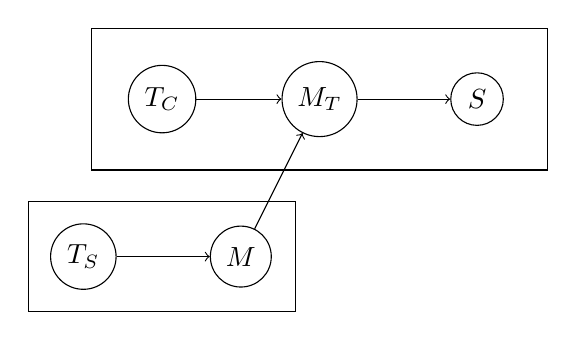
\begin{tikzpicture}
    \node (ts) at (0,0) [circle, draw] {$T_S$};
    \node (m) at (2,0) [circle, draw] {$M$};
    \node (tc) at (1,2) [circle, draw] {$T_C$};
    \node (mt) at (3,2) [circle, draw] {$M_T$};
    \node (s) at (5,2) [circle, draw] {$S$};

    \draw[->] (ts) -- (m);
    \draw[->] (tc) -- (mt);
    \draw[->] (m) -- (mt);
    \draw[->] (mt) -- (s);

    \draw (-.7,-.7) rectangle (2.7,.7);
    \draw (0.1,1.1) rectangle (5.9,2.9);
  \end{tikzpicture}

  \caption{Model for sentiment detection}
  \label{fig:casestudy-sentimentmodel}
\end{figure}

\section{Comparing sentiment time series with share prices}
\label{s:casestudy-comparison}